\documentclass[a4paper,UTF8]{ctexart}

\usepackage{amsmath, amsthm, amssymb, amsfonts, hyperref, mathrsfs}%美国数学学会的包+?
\usepackage{geometry} %控制界面
\usepackage{bookmark}
\usepackage{fancyhdr} % header & footer
\usepackage{appendix} % 附录
\usepackage{tikz} %作图
\usepackage{graphicx} %插入图片的宏包
\usepackage{float} %设置图片浮动位置的宏包
%\usepackage{subfigure} %插入多图时用子图显示的宏包
\usepackage{listings} %引用代码
\usepackage{physics,mathtools} %物理数学工具
\usepackage{comment}
\usepackage{framed}
\usepackage{caption}
\usepackage{subcaption}
\geometry{top=2.5cm,bottom=2.5cm,left=2.5cm,right=2.5cm} % 布局要求
\pagestyle{fancy} % fancy分格
\fancyhf{} % 清除所有页眉页脚
\renewcommand\headrulewidth{0.6pt}
\renewcommand\footrulewidth{0.6pt}
% font
\setCJKmainfont{Noto Serif CJK SC}[BoldFont={Noto Serif CJK SC Bold}, ItalicFont=]
\lhead{何金铭 PB21020660$\mid$座位号:6}
\chead{磁光效应系列测量实验报告}
\rhead{\thepage}
\lfoot{2024.4.11}
\rfoot{USTC}
%\bibliographystyle{plain} % 引用样式
\everymath{\displaystyle} % display
%============================================================

\begin{document}

\begin{center}
    \textbf{\Large 磁光效应系列测量实验报告}
    \par \text{\large 何金铭 PB21020660}
\end{center}

实验目的,实验原理,实验内容已于预习报告中给出,于此报告中不再复述。

\section{实验结果与分析}

检偏器一共转动了30格,一圈对应了50格,三圈对应了$5^{\circ}$,故检偏器一共转过$\delta = 1^{\circ}$

外加磁场$B$可以用外加电流$I$来表示,磁化强度可以用光强即光电探测器读数$U$来表示。
通过改变电流$I$从$0A \rightarrow 3A \rightarrow 0A \rightarrow -3A \rightarrow 0A \rightarrow 3A$,
记录相应的光电探测器读数$U$,得下面的记录表
\begin{table}[H]
    \centering
    \caption{磁滞回线记录表}
    \begin{tabular}{|l|l|l|l|l|l|l|l|}
    \hline
        $I/A$ & 0 & 0.2 & 0.4 & 0.6 & 0.8 & 1 & 1.2 \\ \hline
        $U/V$ & 0.1316 & 0.1318 & 0.1332 & 0.1345 & 0.1354 & 0.1372 & 0.1382 \\ \hline
        $I/A$ & 1.4 & 1.6 & 1.8 & 2 & 2.2 & 2.4 & 2.6 \\ \hline
        $U/V$ & 0.1392 & 0.1394 & 0.141 & 0.1421 & 0.1433 & 0.1451 & 0.147 \\ \hline
        $I/A$ & 2.8 & 3 & 2.8 & 2.6 & 2.4 & 2.2 & 2 \\ \hline
        $U/V$ & 0.1473 & 0.148 & 0.1478 & 0.1474 & 0.1472 & 0.1459 & 0.1445 \\ \hline
        $I/A$ & 1.8 & 1.6 & 1.4 & 1.2 & 1 & 0.8 & 0.6 \\ \hline
        $U/V$ & 0.1432 & 0.1416 & 0.1399 & 0.1389 & 0.1376 & 0.1359 & 0.1346 \\ \hline
        $I/A$ & 0.4 & 0.2 & 0 & -0.2 & -0.4 & -0.6 & -0.8 \\ \hline
        $U/V$ & 0.1333 & 0.1327 & 0.132 & 0.1301 & 0.1308 & 0.13 & 0.1295 \\ \hline
        $I/A$ & -1 & -1.2 & -1.4 & -1.6 & -1.8 & -2 & -2.2 \\ \hline
        $U/V$ & 0.1285 & 0.1275 & 0.1272 & 0.1255 & 0.1251 & 0.1244 & 0.1235 \\ \hline
        $I/A$ & -2.4 & -2.6 & -2.8 & -3 & -2.8 & -2.6 & -2.4 \\ \hline
        $U/V$ & 0.1221 & 0.1211 & 0.1205 & 0.1203 & 0.1212 & 0.1216 & 0.1222 \\ \hline
        $I/A$ & -2.2 & -2 & -1.8 & -1.6 & -1.4 & -1.2 & -1 \\ \hline
        $U/V$ & 0.1227 & 0.1237 & 0.1248 & 0.1263 & 0.1267 & 0.1274 & 0.1286 \\ \hline
        $I/A$ & -0.8 & -0.6 & -0.4 & -0.2 & 0 & 0.2 & 0.4 \\ \hline
        $U/V$ & 0.1299 & 0.1308 & 0.1318 & 0.1332 & 0.134 & 0.1351 & 0.1359 \\ \hline
        $I/A$ & 0.6 & 0.8 & 1 & 1.2 & 1.4 & 1.6 & 1.8 \\ \hline
        $U/V$ & 0.1378 & 0.1385 & 0.1391 & 0.1398 & 0.1403 & 0.1414 & 0.1422 \\ \hline
        $I/A$ & 2 & 2.2 & 2.4 & 2.6 & 2.8 & 3 & ~ \\ \hline
        $U/V$ & 0.1432 & 0.1445 & 0.1456 & 0.1469 & 0.1479 & 0.148 & ~ \\ \hline
    \end{tabular}
\end{table}

可以画出磁滞回线的图像:

\begin{figure}[H]
    \centering
    \begin{minipage}[b]{0.9\textwidth}
        \centering
        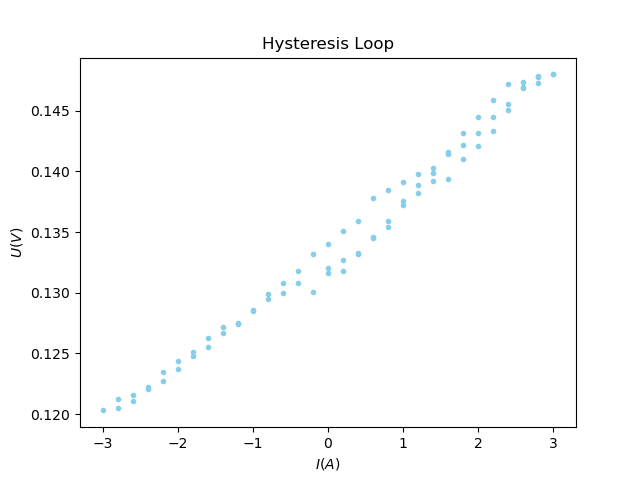
\includegraphics[width=0.9\textwidth]{./1.png}
        \caption{测得的磁滞回线}
    \end{minipage}
\end{figure}

可通过下式来推得达到磁化饱和状态时的克尔转角$\theta_k$

\begin{equation}
\theta_k=\frac{1}{2}\left(\theta_k^{+}-\theta_k^{-}\right)=\frac{\delta}{4} \frac{I\left(+M_s\right)-I\left(-M_s\right)}{I_0}=\frac{\delta}{4} \frac{\Delta I}{I_0}
\end{equation}

其中$I(+M_s) = 0.148V, I(-M_s) = 0.1203V, I_0 = 0.1316V, \delta = 1^{\circ}$

计算得:$0.0526^{\circ}$

\section{实验结论}

\begin{enumerate}
    \item 实验中利用了磁光效应的原理,测量了镍薄膜的磁光克尔旋转角$\theta_k = 0.0526^{\circ}$
    \item 并给出了样品的磁滞回线如上图所示。
\end{enumerate}

\section{思考题}

\subsection{磁光克尔效应测量实验中,$\delta$的大小该如何选取?如果过大或过小分别会对测量有什么样的影响?}

$\delta$的选取不应过大或过小。

\begin{enumerate}
    \item 若过大,则使得之前的近似条件不再成立,会导致测量结果的相对误差增大。
    \item 若过小,则使得光强的变化不明显,会导致测量结果的相对误差增大。
\end{enumerate}

\subsection{克尔效应测量实验中,加上一定的外加磁场后,反射光束是否还是线偏振光?如何通过
我们的实验设备来判断?}

反射光不再是线偏振光。

转动检偏器一周,若测得的最小光强明显大于光电探测器的背景光强,则说明反射光不再是线偏振光。

\subsection{实验中如何判断克尔转角和法拉第旋转角的旋转方向?写出具体的判断过程。}

记录不加磁场时的光电探测器读数$I_0$,加了磁场后,转动检偏器一个小角度:

\begin{enumerate}
    \item 若测得的光强$I$变大,则代表检偏器转动方向为克尔转角和法拉第转角的旋转方向
    \item 若测得的光强$I$变小,则代表检偏器转动方向为克尔转角和法拉第转角的旋转方向的相反方向
\end{enumerate}

\subsection{法拉第效应测量实验中,起偏格兰棱镜的偏振方向是否需要精细调节,为什么?}

需要进行精细调节。当入射光的偏振方向与起偏格兰棱镜的偏振方向垂直时,样品中的磁场才能够对光产生最大的影响,从而使旋光效应最为显著。如果起偏格兰棱镜的偏振方向与入射光的偏振方向不垂直,将导致测量得的光强变化在加磁场前后不明显,影响费尔德系数的准确性。

\end{document}